\begin{activity} \label{A:9.1.4}
    Let $P=(x_0, y_0, z_0)$ and $Q=(x_1, y_1, z_1)$ be two points in $\R^3$. These two points form opposite vertices of a rectangular box whose sides are planes parallel to the coordinate planes as illustrated in Figure \ref{F:9.1.Distance_3D}, and the distance between $P$ and $Q$ is the length of the diagonal shown in Figure \ref{F:9.1.Distance_3D}.
    \begin{figure}[ht]
\begin{center}
%\resizebox{!}{2.0in}{\includegraphics{figures/9_1_Distance_3D}}
  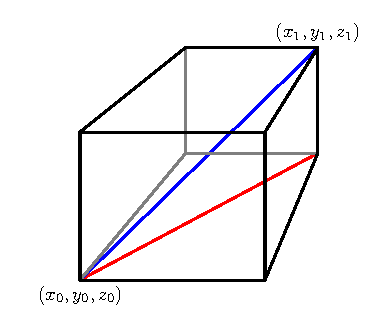
\includegraphics{figures/fig_9_1_distance.eps}
\caption{The distance formula in $\R^3$.}
\label{F:9.1.Distance_3D}
\end{center}
\end{figure}
    \ba
  \item Consider one of the right triangles in the base of the box whose
    hypotenuse is shown as the red line in Figure
    \ref{F:9.1.Distance_3D}. What are the vertices of this triangle?
    Since this right triangle lies in a plane, we can use the
    Pythagorean Theorem to find a formula for the length of the
    hypotenuse of this triangle. Find such a formula, which will be in
    terms of $x_0$, $y_0$, $x_1$, and $y_1$.

  \item Now notice that the triangle whose hypotenuse is the blue segment
    connecting the points $P$ and $Q$ with a leg as the hypotenuse of
    the triangle found in part (a) lies entirely in a plane, so we can
    again use the Pythagorean Theorem to find the length of its
    hypotenuse. Explain why the length of this hypotenuse, which is
    the distance between the points $P$ and $Q$, is
        \begin{equation*} %\label{eq:9.1.Distance_3D}
        \sqrt{(x_1-x_0)^2 + (y_1-y_0)^2 + (z_1-z_0)^2}.
        \end{equation*}

    \ea
\end{activity}
\begin{smallhint}
\ba
\item What are the equations of the faces of the box?
\item What is the distance between the point $Q$ and the point at the lower right corner of the back of the box? 
\ea

\end{smallhint}
\begin{bighint}
\ba
\item The front face of the box has equation $x=x_0$ and the right face of the box has equation $y=y_1$. 
\item What is the distance between the point $Q$ and the point at the lower right corner of the back of the box? 
\ea
\end{bighint}
\begin{activitySolution}
\ba
\item The front face of the box is the $x=x_0$ plane, the back is the $x=x_1$ plane, the bottom is the $z=z_0$ plane, and the right side is the $y=y_1$ plane. So the coordinates of the point at the lower front right of the box are $(x_0,y_1,z_0)$ and the coordinates of the point at the back lower right of the box are $(x_1, y_1, z_0)$. The length of the legs of this triangle are $\mid y_1-y_0\mid$  (the distance between the points $(x_0, y_0, z_0)$ and $(x_0,y_1,z_0)$) and $\mid x_1-x_0 \mid$ (the distance between the points $(x_0, y_1, z_0)$ and $(x_1,y_1,z_0)$). The Pythagorean Theorem then shows that the length of the hypotenuse of the triangle in the base of the box is  
\[\sqrt{(x_1-x_0)^2+(y_1-y_0)^2}.\]
\item The distance between $P$ and $Q$ is the length of the hypotenuse of the triangle whose legs are the hypotenuse of the triangle in the base of the box and whose height is the distance between the points $Q=(x_1,y_1,z_1)$ and $R=(x_1, y_1, z_0)$ (the point at the bottom right corner of the back of the box). The distance between $Q$ and $R$ is just $\mid z_1-z_0\mid$. Using the result from part (a), the Pythagorean Theorem shows that the distance between $P$ and $Q$ is 
\[\sqrt{\left(\sqrt{(x_1-x_0)^2+(y_1-y_0)^2}\right)^2 + (z_1-z_0)^2} = \sqrt{(x_1-x_0)^2 + (y_1-y_0)^2 + (z_1-z_0)^2}\]
as desired.  
\ea
\end{activitySolution}
\aftera 
